%%% Local Variables:
%%% mode: latex
%%% TeX-master: t
%%% End:

\documentclass{article}

\usepackage{fullpage}
\usepackage[utf8]{inputenc}
\usepackage{listings}
\usepackage[table]{xcolor}
\usepackage{amssymb}
\usepackage{amsmath}
\usepackage{fancyhdr}
\usepackage{lastpage}
\usepackage{parskip}
\usepackage{abstract}
\usepackage{url}
\usepackage{float}
\usepackage{enumitem}
\usepackage{fancybox}
\usepackage{amsmath}
\usepackage{graphicx}
\usepackage[bottom]{footmisc}
\usepackage{hyperref}
\usepackage{makecell}


% constants
\newcommand{\COURSE}{02257 Applied Functional Programming}
\newcommand{\TITLE}{Project 2}
\newcommand{\DATE}{January 14, 2015}


%%% Local Variables:
%%% mode: latex
%%% TeX-master: "report"
%%% End:
\newcommand{\code}[1]{\texttt{#1}}
\newcommand{\fn}[2]{\lambda{} \ #1 \mapsto{} #2 }
\newcommand{\ite}[3]{\texttt{ if } #1 \texttt{ then } #2 \texttt{ else } #3 }
\newcommand{\qcol}{\quad:\quad}
\newcommand{\qvd}{\quad\vdash\quad}
%% source / reference
\newcommand{\refgeneral}[3]{#1 (#3), \emph{#2}}
% arguments:
% author
% title
% year
% publisher
\newcommand{\refbook}[4]{\refgeneral{#1}{#2}{#3}, #4}
% arguments:
% author
% title
% year
% url
\newcommand{\refonline}[4]{\refgeneral{#1}{#2}{#3} \\\url{<#4>}}
\definecolor{Brown}{cmyk}{0,0.81,1,0.60}
\definecolor{OliveGreen}{cmyk}{0.64,0,0.95,0.40}
\definecolor{CadetBlue}{cmyk}{0.62,0.57,0.23,0}
\definecolor{lightlightgray}{gray}{0.95}
\definecolor{lightgray}{gray}{0.85}
\definecolor{sh_comment}{rgb}{0.12, 0.38, 0.18}
\definecolor{sh_keyword}{rgb}{0.37, 0.38, 0.75}
\definecolor{sh_string}{rgb}{0.06, 0.10, 0.98}
\lstset{
basicstyle=\small\ttfamily,
stringstyle=\color{sh_string},
keywordstyle = \color{sh_keyword}\bfseries,
commentstyle=\color{sh_comment},
backgroundcolor=\color{lightlightgray},
frame=single,
rulecolor=\color{lightgray},
framesep=3pt,
numbersep=5pt,
xleftmargin=10pt,
xrightmargin=10pt,
showspaces=false,
showstringspaces=false,
tabsize=4,
aboveskip=5pt,
belowskip=5pt,
lineskip=2pt,
captionpos=b,
numbers=left,
numberstyle=\tiny,
stepnumber=1,
numbersep=100pt,
breaklines,
numbersep=5pt,
breakatwhitespace=false,
showspaces=false,
showtabs=false
}
\lstdefinelanguage{llvm}{
morecomment = [l]{;},
morestring=[b]",
sensitive = true,
classoffset=0,
morekeywords={
define, declare, global, constant,
internal, external, private,
linkonce, linkonce_odr, weak, weak_odr, appending,
common, extern_weak,
thread_local, dllimport, dllexport,
hidden, protected, default,
except, deplibs,
volatile, fastcc, coldcc, cc, ccc,
x86_stdcallcc, x86_fastcallcc,
ptx_kernel, ptx_device,
signext, zeroext, inreg, sret, nounwind, noreturn,
nocapture, byval, nest, readnone, readonly, noalias, uwtable,
inlinehint, noinline, alwaysinline, optsize, ssp, sspreq,
noredzone, noimplicitfloat, naked, alignstack,
module, asm, align, tail, to,
addrspace, section, alias, sideeffect, c, gc,
target, datalayout, triple,
blockaddress
},
classoffset=1, keywordstyle=\color{purple},
morekeywords={
fadd, sub, fsub, mul, fmul,
sdiv, udiv, fdiv, srem, urem, frem,
and, or, xor,
icmp, fcmp,
eq, ne, ugt, uge, ult, ule, sgt, sge, slt, sle,
oeq, ogt, oge, olt, ole, one, ord, ueq, ugt, uge,
ult, ule, une, uno,
nuw, nsw, exact, inbounds,
phi, call, select, shl, lshr, ashr, va_arg,
trunc, zext, sext,
fptrunc, fpext, fptoui, fptosi, uitofp, sitofp,
ptrtoint, inttoptr, bitcast,
ret, br, indirectbr, switch, invoke, unwind, unreachable,
malloc, alloca, free, load, store, getelementptr,
extractelement, insertelement, shufflevector,
extractvalue, insertvalue,
},
alsoletter={\%},
keywordsprefix={\%},
}
\lstdefinelanguage{JavaScript}{
keywords={typeof, new, true, false, catch, function, return, null, catch, switch, var, if, in, while, do, else, case, break},
keywordstyle=\color{blue}\bfseries,
ndkeywords={class, export, boolean, throw, implements, import, this},
ndkeywordstyle=\color{darkgray}\bfseries,
identifierstyle=\color{black},
sensitive=false,
comment=[l]{//},
morecomment=[s]{/*}{*/},
commentstyle=\color{purple}\ttfamily,
stringstyle=\color{red}\ttfamily,
morestring=[b]',
morestring=[b]"
}
\makeatother



\lstnewenvironment{promela}[0]{
\lstset{language=C++,
,morekeywords={if, then, else, return, function, var, for, foreach, do, end, od, fi}}
}
{}

\lstnewenvironment{java}[0]{
\lstset{language=C++,
}}
{}

% pseudo code environment
\lstnewenvironment{pseudo}[0]{
\lstset{
language=java
}}
{}


\pagestyle{fancy}
\fancyhf{}
\setlength{\parindent}{0pt}
\setlength{\headheight}{15pt}
\setlength{\headsep}{25pt}
\lhead{\COURSE}
\chead{\TITLE}
\rhead{\DATE}
\cfoot{Page \thepage{} of~\pageref{LastPage}}


\title{\TITLE\\ {\large \COURSE}}
\date{\DATE}
\author{
  Markus Færevaag {\tt s123692}\\
  Simon Altschuler {\tt s123563}
}


\begin{document}
\maketitle
\vspace{10cm}
\doublesignature{Markus Færevaag}{Simon Altschuler} \\
\clearpage


\section{Introduction}
In this report we will describe our experience with porting Andrew Kennedy's SML code to F\# and the corresponding optimizations and PostScript document generation.


\section{Status}
All trees generated by our parser for the While language can be rendered using our program. The renderer has a feature which allows rendering the AST of a (valid) While program file directly.

The generated PostScript document renders the AST in a ``pleasing'' manner, where wide labels do not overlap and connections between nodes are nicely curved.

We have implemented two versions of the PostScript generator, one that uses simple \texttt{sprintf} operations and one that utilizes the \texttt{.NET} \texttt{StringBuilder} for performance optimization. We have analyzed the resulting running time of PostScript generation separately and for the full drill of transforming, designing and rendering an AST.

The only issue known to us is the placement of the generated rendering on the page and more importantly the actual size of the page. It is apparently non trivial to set the generated page size in PostScript, causing large trees to span out of the page.

Following is a very brief description of each task and finally the running time analysis.


\section{Porting to F\#}
Porting the SML code to F\# was fairly straight-forward, with most issues being syntactical differences between the languages.


\section{Transforming the AST}
The transformation of the AST to the general \texttt{Tree} data structure was a simple matter of assigning suitable labels for each type of node, and recursively parsing their children. There are various ways in which one can choose to represent a node such as \texttt{Apply(name, expressions)}, for instance as a pair, a flattened list containing the name and expressions or having the name in the label of the node. We went with the latter.


\section{Avoiding label overlap}
Prevent wide labels from overlapping can be done in either the design phase or when generating PostScript. We chose to do it in the design phase by passing around the label and extending a node's extent accordingly. This is not an optimal solution because we cannot know the width of the label exactly (further complicated by not using a monospace font). It does however work fairly well for this small use case.


\section{Generating PostScript}
PostScript is a plaintext format which means that it is quite easy to generate. We have written some simple functions such as \texttt{drawLabel} and \texttt{drawCurve} that we use as building blocks in the \texttt{drawTree} function. For the simple \texttt{sprintf} version, all the primitive drawing functions are pure, but the \texttt{StringBuilder} version (\texttt{TreeDrawBuilder.fs}) takes, and modifies, a \texttt{StringBuilder} instance instead of returning a string. It is very imperative in style and ruins the elegance, yet it is much faster (see section \ref{sec:analysis} on analysis), and could most likely be refactored into something easier on the mind and eyes.


\section{Analysis}
\label{sec:analysis}
The complexity of the algorithm is $O(n^2)$ where $n$ is the amount AST nodes, but the amortized cost of the program seems close to linear. It is however obvious that the \texttt{StringBuilder} variant is much faster. Figure \ref{fig:plot} visualizes the running times that we recorded on input sizes ranging from 1 node to 400 nodes.

\begin{figure}[H]
  \centering
  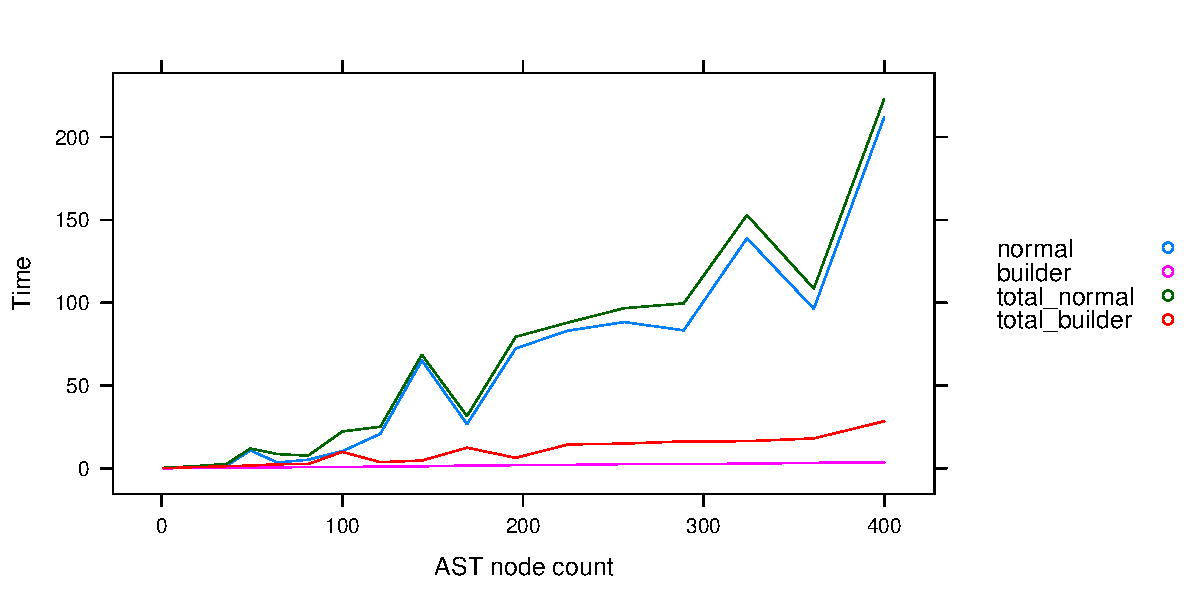
\includegraphics[width=0.8\textwidth]{../times.pdf}
  \caption{Running times compared to amount of AST nodes}
  \label{fig:plot}
\end{figure}

\section{Running the solution}
To generate a drawing simply run the \texttt{Draw.fsx} file. By default it will rendering the \texttt{program/Factorial1.while} file, but that can be easily changed for another file. A file called \texttt{tree.ps} will be generated with the final rendering.

For what it's worth; the analysis can be run by running the \texttt{Analyze.fsx} script, which loads the appropriate tree builder algorithm (either {\tt TreeDraw.fs} for regular strings or {\tt TreeDrawBuilder.fs} for {\tt StringBuilder}).

\end{document}
